\chapter{Methods}
\label{cha:methods}

\section{Core Idea}

\newcommand{\R}{\mathbb{R}}
\newcommand{\E}{\mathbb{E}}
\newcommand{\PG}{\mathrm{PG}}
\newcommand{\xo}{x^o}
\newcommand{\xm}{x^m}

\subsection{Setup} Consider a logistic regression, with missing features in the observation.\\ 
Let $x := (\xo, \xm) \in \R^{d}$. Then the logistic regression is defined as
\[
  p(y \mid x) := \sigma (w^T x), \qquad w \in \R^{d}.
\]
Additionally we have a PC that models the density $p(x)$.

\subsection{Goal} Compute the prediction in a probabilistically principled manner using
\[
  p(y \mid \xo) := \E_{p(\xm \mid \xo)} \left[\sigma \left( w^T x \right) \right].
\]

If it were not for the non-linear sigmoid function $\sigma$, we would be able to calculate this in a smooth 
and decomposable PC, by pulling the Expectation -which is linear- into the leaf nodes. To tackle this we propose to use two tricks.

\subsection{Trick 1: Pólya-Gamma}

To replace the sigmoid function we use the PG-Sigmoid identity, shown in \cite{polyagamma}, that states:

\[
  \sigma(z) = \frac{1}{2} \exp \left(\frac{1}{2}z\right) \
  \E_{\gamma \sim \PG(1,0)} \left[\exp \left(-\frac{1}{2} \gamma z^2 \right)\right]
\]
for $z \in \R$.

If we set $z := w^T x$, and insert into our expectation, we get:
\begin{align*}
  p(y \mid \xo)
  & = \E_{p(\xm \mid \xo)} \left[\sigma(z)\right] \\
  & = \E_{p(\xm \mid \xo)} \left[
       \frac{1}{2}\exp \left(\frac{1}{2}z\right)
       \E_{\gamma \sim \PG(1,0)} \left[\exp \left(-\frac{1}{2}\gamma z^2 \right)\right]
     \right] \\
  & = \frac{1}{2} \E_{p(\xm \mid \xo)} \E_{\gamma \sim \PG(1,0)}
    \left[ \exp \left(\frac{1}{2}z - \frac{1}{2}\gamma z^2 \right) \right]
\end{align*}

Intuitively, this means the sigmoid is replaced with a lot of bell-shaped curves averaged together, one for every value of $\gamma$. 
Figure~\ref{fig:pcpg-bells} shows how well different number of bells approximate $\sigma$.

\begin{figure}[htb]
  \centering
  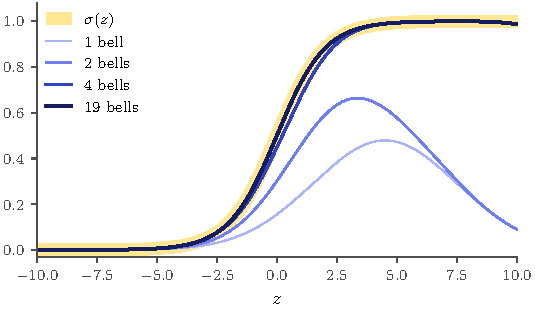
\includegraphics[width=0.75\textwidth]{figures/pcpg/bells.pdf}
  \caption[The Pólya-Gamma identity]{The Pólya-Gamma identity graphically.
    The sigmoid represented as an average of bells
    $\sigma(z) = \E_{\gamma} \left[ \frac{1}{2} e^{\frac{z}{2} - \frac{\gamma z^2}{2}} \right]$.}
  \label{fig:pcpg-bells}
\end{figure}

Now, we have a term without a sigmoid, but the $x$ still appears in a quadratic form.

\subsection{Trick 2: Hubbard-Stratonovich (HS)}

To get rid of the quadratic form, we apply the Hubbard--Stratonovich identity \cite{stratonovich1957, hubbard1959}, that states:

\begin{equation}
    \exp \left( -\tfrac{1}{2} a h^2 \right) = \sqrt{  \frac{1}{2 \pi a}} \int_{-\infty}^{\infty} \exp \left(-\frac{u^2}{2a} -i h u\right) \mathrm{d}u,
\end{equation}

Since $\frac{1}{\sqrt{2\pi a}}\exp\!\left(-\frac{u^2}{2a}\right)$ is the density of $\mathcal{N}(0,a)$, the integral is
exactly the expectation of $e^{-ihu}$ over $u \sim \mathcal{N}(0,a)$:
\begin{equation}
    \exp \left( -\tfrac{1}{2} a h^2 \right) = \E_{u \sim \mathcal{N}(0,\,a)}\!\left[ e^{-ihu} \right].
\end{equation}

The trick makes a quadratic term linear at the cost of introducing a helper variable that we need to integrate over. 
In our term, $x$ appears quadratically as well as linearly. To be able to apply HS, we complete the square (again using $z = w^T x$), where we write $c := \frac{1}{2\gamma}$:

\begin{align}
  \frac{1}{2}z - \frac{1}{2}\gamma z^2
  &= -\frac{1}{2}\gamma \left(z^2 - \frac{z}{\gamma}\right) \notag\\
  &= -\frac{1}{2}\gamma \left(z^2 - 2cz\right) \notag\\
  &= -\frac{1}{2}\gamma \left(\left(z - c\right)^{2} - c^2\right) \notag\\
  &= -\frac{1}{2}\gamma \left(z - c\right)^{2} + \frac{1}{2}\gamma c^2 \notag\\
  &= -\frac{1}{2}\gamma \left(z - c\right)^{2} + \frac{1}{8\gamma}.
\end{align}

Now we apply HS with $a = \gamma$ and $h = z - c$:

\begin{align}
  \exp \left(\frac{1}{2}z - \frac{1}{2}\gamma z^2 \right)
  &= \exp \left(\frac{1}{8\gamma}\right) \exp \left(-\frac{1}{2} \gamma \left(z - c\right)^{2} \right) \notag \\
  &= \exp \left(\frac{1}{8\gamma}\right) \E_{u \sim \mathcal{N}(0, \gamma)} \left[ \exp \left(-iu \left(z - c\right) \right) \right]
\end{align}

Substituting back into $p(y \mid \xo)$, we get:

\begin{align*}
  p(y \mid \xo)
  &= \frac{1}{2} \E_{p(\xm \mid \xo)} \E_{\gamma \sim \PG(1,0)} \left[ \exp \left(\frac{1}{2}z - \frac{1}{2}\gamma z^2 \right) \right] \\
  &= \frac{1}{2} \E_{p(\xm \mid \xo)} \E_{\gamma \sim \PG(1,0)} \left[ \exp \left(\frac{1}{8\gamma}\right) \E_{u \sim \mathcal{N}(0, \gamma)} \left[ \exp \left(-iu \left(z - c\right) \right) \right] \right]
\end{align*}

Intuitively, this means every bell is replaced with a lot of cosine waves $\cos(u(z - c))$ averaged together, one for every value of $u$ (see Appendix~\ref{app:waves} for the derivation).
Figure~\ref{fig:pcpg-waves} shows how well different numbers of waves approximate a bell.

\begin{figure}[htb]
  \centering
  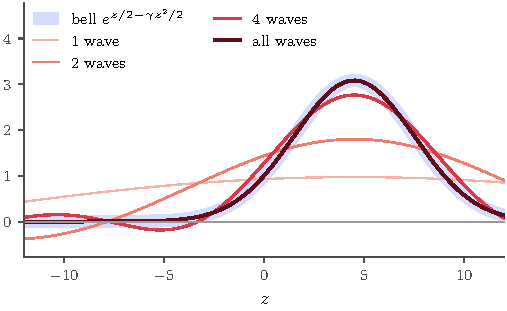
\includegraphics[width=0.75\textwidth]{figures/pcpg/waves.pdf}
  \caption[The Hubbard-Stratonovich identity]{The Hubbard-Stratonovich identity graphically.
    A bell from Figure~\ref{fig:pcpg-bells} represented as an average of waves
    $e^{-\frac{\gamma}{2}(z - c)^2}$.}
  \label{fig:pcpg-waves}
\end{figure}

\subsection{Arriving at the Characteristic Function}

To continue, we want the expectation over $\xm$ to be the innermost one, so we swap the order of the expectations:
\[
  p(y \mid \xo) = \frac{1}{2} \E_{\gamma \sim \PG(1,0)} \E_{u \sim \mathcal{N}(0, \gamma)} \left[ \exp \left(\frac{1}{8\gamma}\right) \E_{p(\xm \mid \xo)} \left[ \exp \left(-iu \left(z - c\right) \right) \right] \right].
\]
This is allowed because \dots

The innermost expectation is now only over $\xm$, with $\xo$ fixed, so we split $z = w^T x$ into its observed and missing parts:
\[
  z = w^T x = w_o^T \xo + w_m^T \xm.
\]

The $\xo$ part and $c$ are constant under $\E_{p(\xm \mid \xo)}$ and factor out:
\begin{align*}
  \E_{p(\xm \mid \xo)} \left[ \exp \left(-iu \left(z - c\right) \right) \right]
  &= \E_{p(\xm \mid \xo)} \left[ \exp\left(-iu \left(w_o^T \xo - c + w_m^T \xm\right)\right) \right] \\
  &= \exp\left(iu \left(c - w_o^T \xo\right)\right) \cdot \E_{p(\xm \mid \xo)} \left[ \exp\left(-iw_m^T \xm u\right) \right]
\end{align*}

This remaining expectation is a known quantity: the characteristic function of a random variable $X$,
$\phi_X(s) := \E \left[ \exp(i s^T X) \right]$. Writing $-iw_m^T \xm u = i(-uw_m)^T \xm$, we get:

\[
  \E_{p(\xm \mid \xo)} \left[ \exp \left(-iu \left(z - c\right) \right) \right] = \exp\left(iu \left(c - w_o^T \xo\right)\right) \cdot \phi_{\xm \mid \xo}(-uw_m).
\]

Intuitively, the characteristic function gives the expectation of a wave under the distribution $p(z)$ of $z = w^T x$: for every frequency $u$, it gives the signed area under the wave times $p(z)$ (see Appendix~\ref{app:cf-area} for the derivation).
Figure~\ref{fig:pcpg-cf} shows this for two different waves, i.e.\ different values of $u$.

\begin{figure}[htb]
  \centering
  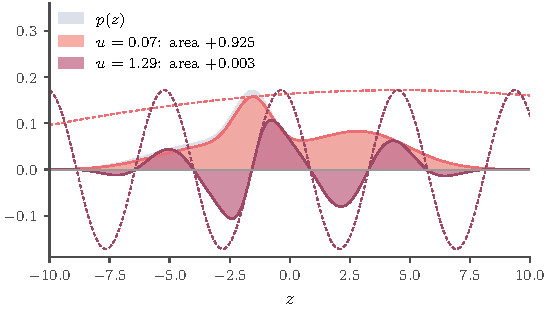
\includegraphics[width=0.75\textwidth]{figures/pcpg/cf.pdf}
  \caption[The characteristic function]{The characteristic function graphically.
    The expectation of a wave under $p(z)$ is the signed area under the wave times $p(z)$ (shaded). Fast waves average to zero, while slower waves give a non-zero value.}
  \label{fig:pcpg-cf}
\end{figure}

\subsection{Full Formula}

Plugging the result of the previous subsection into $p(y \mid \xo)$ and writing out $c = \frac{1}{2\gamma}$, we obtain:
\begin{align*}
  p(y \mid \xo)
  &= \frac{1}{2} \E_{p(\xm \mid \xo)} \E_{\gamma \sim \PG(1,0)} \left[ \exp \left(\frac{1}{8\gamma}\right) \E_{u \sim \mathcal{N}(0, \gamma)} \left[ \exp \left(-iu \left(z - c\right) \right) \right] \right] \\
  &= \frac{1}{2} \E_{\gamma \sim \PG(1,0)} \E_{u \sim \mathcal{N}(0, \gamma)} \left[ \exp \left(\frac{1}{8\gamma}\right) \exp\left(iu \left(\frac{1}{2\gamma} - w_o^T \xo\right)\right) \phi_{\xm \mid \xo}(-uw_m) \right]
\end{align*}

We propose this as a final expression that we can tractably evaluate.

\subsection{Summary}

The expected prediction $p(y \mid \xo)$ is the area under $\sigma(z)\, p(z)$. 
We replace the sigmoid function by a sum of weighted bells. We get the area under each weighted bell times $p(z)$,
by replacing each bell with a sum of waves and put each wave frequency into the characteristic function, which gives the
signed area under the wave times $p(z)$. 

\begin{figure}[htb]
  \centering
  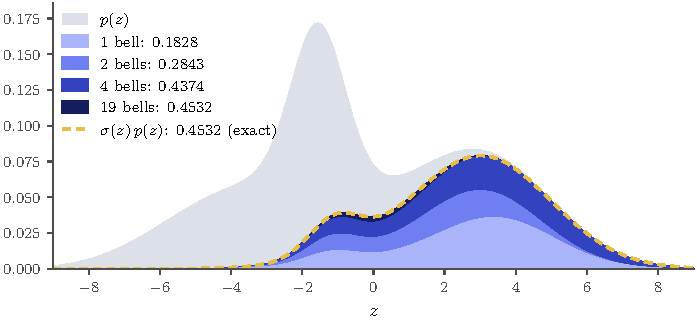
\includegraphics[width=\textwidth]{figures/pcpg/summary.pdf}
  \caption[The expected prediction as a sum of bells]{The expected prediction as a sum of bells.
    $p(y \mid \xo)$ is the area under $\sigma(z)\, p(z)$ (dashed).
    Adding up the areas under the weighted bells times $p(z)$ (shaded), each computed from the characteristic function, recovers it.}
  \label{fig:pcpg-summary}
\end{figure}

\section{Calculating the Two Expectations}
\label{sec:approx}

After the two tricks, $p(y \mid \xo)$ is an expectation over two variables, $\gamma$ and $u$. There is no closed form solution 
for this, so we need to approximate it. There are multiple ways to do this, but in all the principle is the same:
we take a set of points (nodes) and associated weights, and replace the expectation with a weighted sum. 

We write $f(u, \gamma)$ for the term inside the expectations,
\[
  f(u, \gamma) := \exp \left(\frac{1}{8\gamma}\right) \exp\left(iu \left(\frac{1}{2\gamma} - w_o^T \xo\right)\right) \phi_{\xm \mid \xo}(-uw_m).
\]

\subsection{Monte Carlo}
\label{subsec:pcpg-mc}

The simplest way is to sample both expectations.
We draw $M$ samples $\gamma_j \sim \PG(1,0)$, and for every $\gamma_j$ we draw $N$ samples $u_{ij} \sim \mathcal{N}(0, \gamma_j)$:
Each sample is weighted equally here, so the weights are $w_j = \frac{1}{M}$ and $\omega_{ij} = \frac{1}{N}$. 
Since they are not dependent on the sampled values, we can write them outside the sums. The resulting estimator is

\[
  p(y \mid \xo) \approx \frac{1}{2} \cdot \frac{1}{M} \sum_{j=1}^{M} \frac{1}{N} \sum_{i=1}^{N} f(u_{ij}, \gamma_j).
\]

This is always unbiased, but the variance can be quite high and we need a large number of samples to get a good estimate.

\subsection{Numerical Integration}
\label{subsec:pcpg-quad}

Both expectations can also be computed by quadrature / numerical integration. 
The idea is, that instead of having to choose many points and weights randomly to get an acceptable error, 
we strategically choose a fixed set of specific points and weights that guarantees a certain level of accuracy. 

\subsubsection{Inner Expectation: Gauss--Hermite}
\label{subsec:gauss-hermite}

The inner expectation is over $u \sim \mathcal{N}(0, \gamma)$.  This is an exact case for a standard Gauss--Hermite quadrature (Section~\ref{subsec:bg-gauss-hermite}).

(Should this be explained in more detail?)
We can easily get the nodes $t_i$ and weights $\omega_i$ with \texttt{numpy.polynomial.hermite.hermgauss(N)}, which returns the $N$ nodes and weights for the standard normal distribution $\mathcal{N}(0, 1)$.
We then scale the nodes by $\sqrt{2\gamma}$ and the weights by $\frac{1}{\sqrt{\pi}}$ to transform them for our distribution.

\[
  \E_{u \sim \mathcal{N}(0, \gamma)}[f(u, \gamma)] \approx \frac{1}{\sqrt{\pi}} \sum_{i=1}^{N} \omega_i\, f\!\left(\sqrt{2\gamma}\,t_i, \gamma\right).
\]
Plugging this into the full formula gives
\[
  p(y \mid \xo) \approx \frac{1}{2\sqrt{\pi}} \E_{\gamma \sim \PG(1,0)} \left[ \sum_{i=1}^{N} \omega_i\, f\!\left(\sqrt{2\gamma}\,t_i, \gamma\right) \right].
\]

\subsubsection{Outer Expectation: Gauss--PG}
\label{subsec:pg-quadrature}

While for the inner expectation we can use a standard and widely known quadrature rule, 
there is no standard quadrature rule for an expectation over $\gamma \sim \PG(1,0)$. 
So we need to construct one ourselves. We do this by using the Golub--Welsch algorithm (Section~\ref{subsec:bg-golub-welsch}), 
which is the default choice to construct quadrature nodes and weights for Gauss quadratures.

The Golub--Welsch algorithm only needs the moments of the distribution. For
$\PG(1,0)$ they follow from its Laplace transform
$\mathcal{L}(t) := \E[e^{-t\gamma}] = \operatorname{sech}(\sqrt{t/2})$, which is
known in closed form. Then the $k$-th moment is, the $k$-th derivative
at zero, up to its sign:
\[
  \mu_k := \E[\gamma^k] = (-1)^k\, \mathcal{L}^{(k)}(0).
\]

We then apply the Golub--Welsch procedure and call the rule \emph{Gauss--PG}. It is shown in Algorithm~\ref{alg:gauss-pg}. 

\begin{algorithm}[H]
\caption{Gauss--PG quadrature rule}
\label{alg:gauss-pg}
\begin{algorithmic}[1]
\Require number of nodes $n$
\State compute with 200 digits
\For{$k = 0, \dots, 2n-1$}
  \State $\mu_k \gets (-1)^k\, \mathcal{L}^{(k)}(0)$ with $\mathcal{L}(t) = \operatorname{sech}(\sqrt{t/2})$
\EndFor
\State $H_{ij} \gets \mu_{i+j}$ and $H'_{ij} \gets \mu_{i+j+1}$ for $i, j = 0, \dots, n-1$
\State $R \gets$ Cholesky factor of $H = R^T R$
\State $J \gets R^{-T} H' R^{-1}$
\State $V \Lambda V^T \gets$ eigendecomposition of $J$
\State $\gamma_j \gets \lambda_j$ and $w_j \gets v_{0j}^2$ for $j = 1, \dots, n$
\State \Return $(\gamma_j, w_j)_{j=1}^{n}$
\end{algorithmic}
\end{algorithm}

We do the computation with 200 digits, because the moments only differ very very slightly which makes the Cholesky decomposition fail. 
For regular floating point precision, the moments are already indistinguishable from about $n \geq 12$.

Since $\E[e^{-\gamma z^2/2}] = \mathcal{L}(z^2/2)$, a rule with $n$ nodes
$(\gamma_j, w_j)$ approximates the sigmoid by a sum of bells,
\begin{equation}
  \sigma(z) = \tfrac{1}{2}\, e^{z/2}\, \mathcal{L}\!\left(\tfrac{z^2}{2}\right)
  \approx \tfrac{1}{2}\, e^{z/2} \sum_{j=1}^{n} w_j\, e^{-\gamma_j z^2/2}.
  \label{eq:sigma-laplace}
\end{equation}
Gauss--PG keeps its nodes away from $\gamma = 0$, so the factor
$e^{1/(8\gamma_j)}$ in $f$ stays small. Rules with nodes
closer to zero can approximate the sigmoid \emph{alone} more accurately, but fail with PCPG, becasue the
factor blows up their error. These and other rules for the outer integral are
described in Appendix~\ref{app:pg-rules}.

Combining the Gauss--PG nodes $(\gamma_j, w_j)_{j=1}^{M}$ with the Gauss--Hermite
nodes $(t_i, \omega_i)_{i=1}^{N}$ yields the fully deterministic approximation
\[
  p(y \mid \xo) \approx \frac{1}{2\sqrt{\pi}} \sum_{j=1}^{M} w_j \sum_{i=1}^{N} \omega_i\, f\!\left(\sqrt{2\gamma_j}\,t_i, \gamma_j\right).
\]

\subsubsection{Sign Flip}
\label{subsec:sign-flip}

Like it is somewhat visible in \ref{fig:pcpg-bells}, for $z < 0$ the bells approximate the sigmoid quite well, even a small number of bells.
For $z > 0$ it becomes harder and for larger z, i.e. $z > 10$, the sigmoid is very close to $1$, whereas the sum of bells, no matter how many,
tends towards $0$ eventually. So we'd have a constant error of $1$ for large $z$. More detail in (Appendix~\ref{app:large-z}).

To mitigate this we use that the sigmoid is point symmetric around $(0, \tfrac{1}{2})$:
\[
  \sigma(-z) = \frac{1}{1 + e^{z}} = \frac{e^{-z}}{e^{-z} + 1} = 1 - \sigma(z).
\]

For $z > 0$ we can therefore compute $1 - \hat\sigma(-z)$ instead of $\hat\sigma(z)$.
Both use the same nodes and the same approximation of $\mathcal{L}(z^2/2)$. The error
at $z$ becomes the error at $-z$. In practice this reduces the error over $|z| \leq 30$ of
Gauss--PG with 20 nodes from about $1$ to $6 \cdot 10^{-7}$.

The symmetry can be used for the whole expectation as well,
\[
  \E\bigl[\sigma(w^T x) \mid \xo\bigr] = 1 - \E\bigl[\sigma(-w^T x) \mid \xo\bigr],
\]
which means the estimator can run with $-w$ and return one minus the result. 

Since $z = w^T x$, with some $x$ missing, is random, wether to flip is decided by the sign of
the expected value $\E[w^T x \mid \xo] = w_o^T \xo + w_m^T \E[\xm \mid \xo]$. We do
this for every point individually.

Since the expectation $\E[\xm \mid \xo]$ is available in closed form for GMMs and PCs, we can compute it efficiently and it doesn't 
add much additional cost.

\section{The Characteristic Function of the Density Model}
\label{sec:density-cf}

The only place where the density model is used in PCPG is the conditional
characteristic function $\phi_{\xm \mid \xo}$. In this section we describe how to compute it for the two
density models we use, GMMs and PCs.

\subsection{Gaussian Mixture Models}
\label{subsec:gmm-cf}

For a Gaussian $X \sim \mathcal{N}(\mu, \Sigma)$, the characteristic function
is known in closed form,
\[
  \phi_X(s) = \E\left[\exp(i s^T X)\right] = \exp \left( i s^T \mu - \tfrac{1}{2} s^T \Sigma s \right).
\]

A GMM has the density $p(x) = \sum_{k=1}^{K} \pi_k\, \mathcal{N}(x; \mu_k, \Sigma_k)$.
Since the expectation is linear, the characteristic function of a
mixture is just a mixture of the characteristic functions of its components,
\[
  \phi_X(s) = \sum_{k=1}^{K} \pi_k\, \exp \left( i s^T \mu_k - \tfrac{1}{2} s^T \Sigma_k s \right).
\]

However, in PCPG we need the conditional characteristic function $\phi_{\xm \mid \xo}$, so the
characteristic function of the missing features given the observed ones. To get it, we
first need the conditional density $p(\xm \mid \xo)$, which with diagonal covariances, is the mixture:
\[
  p(\xm \mid \xo) = \sum_{k=1}^{K} \tilde{\pi}_k(\xo)\, \mathcal{N}(\xm; \mu_k^m, \Sigma_k^m),
\]
with the responsibilities
\[
  \tilde{\pi}_k(\xo) = p(k \mid \xo) = \frac{\pi_k\, \mathcal{N}(\xo; \mu_k^o, \Sigma_k^o)}{\sum_{j=1}^{K} \pi_j\, \mathcal{N}(\xo; \mu_j^o, \Sigma_j^o)}.
\]

Its components are the original ones restricted to the missing features, with
mean $\mu_k^m$ and covariance $\Sigma_k^m$. The responsibilities are the posterior
weights for each component. They state how well each component explains the
observed features.

The conditional characteristic function is then just the characteristic function of the conditional mixture, so
\[
  \phi_{\xm \mid \xo}(s) = \sum_{k=1}^{K} \tilde{\pi}_k(\xo) \, \exp \left( i s^T \mu_k^m - \tfrac{1}{2} s^T \Sigma_k^m s \right).
\]

We compute this for every point $\xo$ once and reuse it for all frequencies $s$, since 
the responsibilities $\tilde{\pi}_k(\xo)$ only depend on the observed features.
This is shown in algorithm~\ref{alg:gmm-cf}.

\begin{algorithm}[H]
\caption{Conditional characteristic function of a GMM}
\label{alg:gmm-cf}
\begin{algorithmic}[1]
\Require GMM parameters $\{\pi_k, \mu_k, \Sigma_k\}_{k=1}^{K}$ with diagonal $\Sigma_k = \mathrm{diag}(\sigma_k^2)$, partial observation $\xo$, frequencies $s_1, \dots, s_L$ over the missing features
\For{$k = 1, \dots, K$}
  \State $\tilde{\pi}_k \gets \dfrac{\pi_k \, \mathcal{N}(\xo;\mu_k^o,\Sigma_k^o)}{\sum_{j}\pi_j \,\mathcal{N}(\xo;\mu_j^o,\Sigma_j^o)}$
\EndFor
\For{$l = 1, \dots, L$}
  \State $\phi_l \gets \sum_{k=1}^{K} \tilde{\pi}_k \exp \left( i s_l^T \mu_k^m - \tfrac{1}{2} \sum_{d \in \mathrm{mis}} s_{ld}^2\, \sigma_{kd}^2 \right)$
\EndFor
\State \Return $\phi_1, \dots, \phi_L$
\end{algorithmic}
\end{algorithm}

\subsection{Probabilistic Circuits}
\label{subsec:pc-cf}

How to compute the CF of a general PC.

PC frameworks usually don't provide a method for it. So we need to implement it ourselves. 

The framework SPFlow already offers conditional sampling so we would only need to implement the CF. 
The framework cirkit doesn't have either. 

The PC would also need to be able to give the means of z for the flip.

We could also implement a very simple PC from scratch?

\section{PCPG Algorithm}
\label{sec:algorithm}

Putting everything together leads to the PCPG algorithm shown in Algorithm~\ref{alg:pcpg}. 
For one test point, it decides the sign flip, evaluates the density's conditional characteristic function
at the frequencies given by the nodes, and returns the weighted sum of $f$. 
The Gauss--Hermite and Gauss--PG nodes depend
neither on the point nor on the classifier or the density model, so they are
computed once beforehand. The density model is only used through its characteristic function, 
so the algorithm works for every model that can expose one.

\begin{algorithm}[H]
\caption{PCPG}
\label{alg:pcpg}
\begin{algorithmic}[1]
\Require LR weights $w$, partial observation $\xo$, density model with conditional characteristic function $\phi_{\xm \mid \xo}$, Gauss--PG nodes and weights $(\gamma_j, w_j)_{j=1}^{M}$, Gauss--Hermite nodes and weights $(t_i, \omega_i)_{i=1}^{N}$
\State Split $w = (w_o, w_m)$ by the observed/missing mask
\State $\mathrm{flip} \gets \E[w^T x \mid \xo] > 0$
\If{$\mathrm{flip}$}
  \State $w_o \gets -w_o$, \quad $w_m \gets -w_m$
\EndIf
\State $u_{ij} \gets \sqrt{2\gamma_j}\, t_i$ for all $i, j$
\State $\phi_{ij} \gets \phi_{\xm \mid \xo}(-u_{ij}\, w_m)$ for all $i, j$
\State $S \gets \sum_{j=1}^{M} \sum_{i=1}^{N} w_j\, \omega_i \exp \left(\dfrac{1}{8\gamma_j}\right) \exp\left(i u_{ij} \left(\dfrac{1}{2\gamma_j} - w_o^T \xo\right)\right) \phi_{ij}$
\State $p \gets \dfrac{1}{2\sqrt{\pi}}\, \mathrm{Re}(S)$
\State \Return $1 - p$ if $\mathrm{flip}$, else $p$
\end{algorithmic}
\end{algorithm}

One can come up with other variants of PCPG by changing how the two
expectations are computed. The inner, the outer, or both could be sampled
instead. For both also different quadrature rules could be used. 
Appendix~\ref{app:variants} lists different combinations. In the rest of this thesis, \emph{PCPG} refers to
Algorithm~\ref{alg:pcpg}, and \emph{PCPG-MC} to the variant that samples both
expectations.

\section{Training with PCPG}
\label{sec:training-pcpg}

Up to now, the classifier $w$ was trained on complete data and features were only
missing at test time. However, in practice, training data could also have missing features.

In this section we show how PCPG can also be used in training.

\subsection{Fitting the density}

The density model $p(x)$ is fit first. Here PCPG is not needed, and in general 
this is a standard and well-established procedure. 
The density is fit, by maximizing the marginal likelihood of the observed features $\xo$:

\[
  p(\xo) = \int p( x = (\xo, \xm)) \, \mathrm{d}\xm.
\]

In general this integral is hard, but can be computed tractably for a GMM or a PC. 

For a GMM, we can see this one component $k$ at a time. A component is a
Gaussian $\mathcal{N}(\mu_k, \Sigma_k)$, and since our GMM uses diagonal covariances
$\Sigma_k = \mathrm{diag}(\sigma_{k1}^2, \dots, \sigma_{kD}^2)$, 
every feature $d$, within a component, has its own one-dimensional Gaussian with
mean $\mu_{kd}$ and variance $\sigma_{kd}^2$. This means that the features are independent of each other 
within a component. Since the density of independent variables is the product of their individual densities, 
the density of a point x in component k can be written as
\[
  p(x \mid k) = \prod_{d=1}^{D} \mathcal{N}(x_d; \mu_{kd}, \sigma_{kd}^2).
\]

Now when a feature $d$ is missing, integrating over $x_d$ only touches its own
term $\mathcal{N}(x_d; \mu_{kd}, \sigma_{kd}^2)$. 
Because that term is a density, it integrates to one and it can simply be dropped out of the product. 
Then only the terms of the observed features remain,
\[
  p(\xo) = \sum_{k=1}^{K} \pi_k \prod_{d \in \mathrm{obs}} \mathcal{N}(x_d; \mu_{kd}, \sigma_{kd}^2).
\]

A PC works the same way. Its leaves are the one-dimensional densities of single
features, and when the circuit is smooth and decomposable, the integral over a
missing feature can be moved down to its leaves. There the
leaves of the missing features are simply set to one and the circuit is evaluated as
usual.

$p(x)$ is fit once and kept fixed for the remainder of the training process.

\subsection{Fitting the classifier}

When we already have a way to predict with missing data at test time, 
training the classifier with missing data is actually quite simple.
We just use the same prediction method, that we use at test time, 
namely the expected prediction over all plausible values of the missing features:

\[
  p_n = p(y_n = 1 \mid \xo_n) = \E_{p(\xm \mid \xo_n)} \left[ \sigma(w^T x) \right].
\]

As in an standard logistic regression, $w$ should make true labels as likely
as possible. This means we want to maximize the likelihood of true labels, i.e. the probability the classifier assigns to them, or 
equivalently, minimize the negative log-likelihood. This leads to the following loss function:

\begin{equation}
  J(w) = -\frac{1}{n_\mathrm{train}} \sum_{n=1}^{n_\mathrm{train}} \log p(y_n \mid \xo_n) + \frac{1}{2 C n_\mathrm{train}} \lVert w \rVert^2 .
  \label{eq:marginal-likelihood}
\end{equation}

Here $p(y_n \mid \xo_n)$ means the probability of the true label of point $n$: it is
$p_n$ if $y_n = 1$ and $1 - p_n$ if $y_n = 0$:
\[
  \log p(y_n \mid \xo_n) = y_n \log p_n + (1 - y_n) \log (1 - p_n).
\]
This is the familiar binary cross-entropy.

The second term here is the $L_2$ penalty of scikit-learn's logistic regression, with $C = 1$. 
It keeps $w$ from growing without bound and makes the optimum unique. 

As mentioned we compute the expected prediction $p(y_n \mid \xo_n)$ with PCPG,
and use automatic differentiation to compute the gradient $\nabla_w J(w)$ of the loss function. Then 
we can use any gradient-based optimizer, like Adam, and find the optimal $w$.

\subsection{Algorithm}
\label{subsec:training-algorithm}

Algorithm~\ref{alg:training} puts both stages together. First, we fit the density model $p_\theta(x)$, then the classifier starts at
$w = 0$ and is trained by Adam on minibatches. Since the expected predictions of PCPG
can lie slightly outside $[0, 1]$ due to the quadrature error, we
clamp them to $[\varepsilon, 1 - \varepsilon]$.

\begin{algorithm}[H]
\caption{Training a logistic regression with PCPG}
\label{alg:training}
\begin{algorithmic}[1]
\Require incomplete training points $(\xo_n, y_n)_{n=1}^{n_\mathrm{train}}$, PCPG nodes and weights, penalty $C$, epochs $E$, batch size $B$, learning rate $\eta$, $\varepsilon$
\State Fit the density model: $\theta \gets \arg\max_\theta \sum_{n} \log p_\theta(\xo_n)$
\State $w \gets 0$
\For{$e = 1, \dots, E$}
  \For{every minibatch $\mathcal{B}$ of $B$ training points, in random order}
    \For{$n \in \mathcal{B}$}
      \State $p_n \gets$ PCPG$(w, \xo_n)$ with Algorithm~\ref{alg:pcpg}, clamped to $[\varepsilon, 1 - \varepsilon]$
    \EndFor
    \State $J \gets -\frac{1}{B} \sum_{n \in \mathcal{B}} \left( y_n \log p_n + (1 - y_n) \log (1 - p_n) \right) + \frac{1}{2 C n_\mathrm{train}} \lVert w \rVert^2$
    \State $g \gets \nabla_w J$
    \State $w \gets \mathrm{Adam}(w, g, \eta)$
  \EndFor
\EndFor
\State \Return $w$ and $p_\theta$
\end{algorithmic}
\end{algorithm}

\section{A Direct Route for Gaussian Mixtures}
\label{subsec:gmm-direct}

Although we use GMMs as density models for PCPG throughout, for a GMM the two
tricks are actually not needed: the expected prediction can be computed directly.
We include them anyway, to demonstrate the general approach in a simpler setting and to be 
able to compare the results of PCPG with a reference.

In this section we show how the expected prediction can be computed directly for a GMM.

\subsection{Reducing the Integral to One Dimension}

The prediction $\sigma(w^T x)$ does't depend on individual features, but only
on the single number
\[
  z = w^T x = w_o^T \xo + w_m^T \xm.
\]

The observed part $w_o^T \xo$ is fixed. Only the missing part is random. So
instead of averaging $\sigma$ over all missing features, we can average it just over
$z$, and that is always a one-dimensional number.
This reduces the dimensionality of the integral from the number of missing
features to one, which makes it much easier to compute.
The only thing we need for this is the distribution $p(z \mid \xo)$.

\subsection{The Distribution of $z$}

For a GMM, the distribution of $z$ is relatively easy to find. 

Let's first rewrite $z$ as,

\[
  z = w_o^T \xo + \sum_{d \in \mathrm{mis}} w_d\, x_d,
\]

where the only uncertain part is the sum of the missing features.

Then recall that every missing feature is a one-dimensional Gaussian of its own, and the missing
features are independent of each other,
\[
  x_d \mid k \sim \mathcal{N}(\mu_{kd}, \sigma_{kd}^2) \quad \text{for every } d \in \mathrm{mis}.
\]

A weighted sum of independent Gaussians is again Gaussian. So within component $k$, $z$ is Gaussian as well,
$z \mid k \sim \mathcal{N}(m_k, v_k)$, and we only need its mean $m_k$ and its
variance $v_k$.

The mean of a sum is the sum of the means, and the mean of $w_d x_d$ is
$w_d \mu_{kd}$. So the mean of $z$ is $z$ with every missing feature replaced by
its mean,
\[
  m_k = \E[z \mid k] = c + \sum_{d \in \mathrm{mis}} w_d\, \E[x_d \mid k] = w_o^T \xo + \sum_{d \in \mathrm{mis}} w_d\, \mu_{kd}.
\]

Similarly, the variance of their sum is the sum of their
variances, and multiplying $x_d$ by $w_d$ multiplies its variance by $w_d^2$. So
\[
  v_k = \mathrm{Var}[z \mid k] = \sum_{d \in \mathrm{mis}} \mathrm{Var}[w_d\, x_d \mid k] = \sum_{d \in \mathrm{mis}} w_d^2\, \sigma_{kd}^2.
\]

Lastly, we don't  know which component the point comes from. Every component
gives its own Gaussian for $z$, and the observed features tell us how likely each
component is, through the responsibilities $\tilde{\pi}_k(\xo)$ of
Section~\ref{subsec:gmm-cf}. The distribution of $z$ is therefore the mixture of
these Gaussians, weighted by the responsibilities,
\[
  p(z \mid \xo) = \sum_{k=1}^{K} \tilde{\pi}_k(\xo)\, \mathcal{N}(z; m_k, v_k).
\]

\subsection{Computing the Expected Prediction}

The expected prediction then splits into one average per component,
\[
  p(y \mid \xo) = \sum_{k=1}^{K} \tilde{\pi}_k(\xo)\, \E_{z \sim \mathcal{N}(m_k, v_k)} \left[ \sigma(z) \right].
\]

Each of these averages is a one-dimensional integral of the sigmoid against a
Gaussian. While it doesn't have a closed form solution, it can be very accurately computed using 
numerical integration, like Gauss-Hermite quadrature (Section~\ref{subsec:gauss-hermite}) or adaptive quadrature using \texttt{scipy.integrate.quad}.

\[
  p(y \mid \xo) \approx \frac{1}{\sqrt{\pi}} \sum_{k=1}^{K} \tilde{\pi}_k(\xo) \sum_{i=1}^{N} \omega_i\, \sigma\!\left( m_k + \sqrt{2 v_k}\, t_i \right).
\]

\subsection{The Inner Expectation in Closed Form}
\label{subsec:gmm-exact-inner}

Need to rewrite.

The mixture $p(z \mid \xo)$ can also be used inside PCPG. After the first trick and
swapping the two expectations, the expected prediction is
\[
  p(y \mid \xo) = \frac{1}{2} \E_{\gamma \sim \PG(1,0)} \E_{z \sim p(z \mid \xo)} \left[ \exp \left(\frac{1}{2}z - \frac{1}{2}\gamma z^2 \right) \right].
\]
PCPG computes the inner expectation over $z$ with the second trick and Gauss--Hermite
quadrature. For a GMM it can be computed exactly instead, because the bell
$\exp(\frac{1}{2}z - \frac{1}{2}\gamma z^2)$ times a Gaussian density is again a
Gaussian, up to a constant.

Within component $k$ we have $z \sim \mathcal{N}(m_k, v_k)$, and we drop the index $k$
for the derivation. Writing out the density, the expectation is
\[
  \E_{z \sim \mathcal{N}(m, v)} \left[ \exp \left(\frac{1}{2}z - \frac{1}{2}\gamma z^2 \right) \right] = \frac{1}{\sqrt{2\pi v}} \int_{-\infty}^{\infty} \exp \left(\frac{1}{2}z - \frac{1}{2}\gamma z^2 - \frac{(z - m)^2}{2v} \right) \mathrm{d}z.
\]
The exponent is quadratic in $z$. We collect its terms by powers of $z$ and write
$a := \gamma + \frac{1}{v}$ and $b := \frac{1}{2} + \frac{m}{v}$:
\begin{align*}
  \frac{1}{2}z - \frac{1}{2}\gamma z^2 - \frac{(z - m)^2}{2v}
  &= -\frac{1}{2}\left(\gamma + \frac{1}{v}\right) z^2 + \left(\frac{1}{2} + \frac{m}{v}\right) z - \frac{m^2}{2v} \\
  &= -\frac{1}{2} a z^2 + b z - \frac{m^2}{2v} \\
  &= -\frac{1}{2} a \left(z - \frac{b}{a}\right)^2 + \frac{b^2}{2a} - \frac{m^2}{2v}.
\end{align*}
The last step completes the square, as in the second trick. The last two terms do not
depend on $z$ and can be taken out of the integral. What remains is the integral of
an unnormalised Gaussian with variance $\frac{1}{a}$, which is
$\sqrt{2\pi / a}$. Therefore
\begin{align*}
  \E_{z \sim \mathcal{N}(m, v)} \left[ \exp \left(\frac{1}{2}z - \frac{1}{2}\gamma z^2 \right) \right]
  &= \frac{1}{\sqrt{2\pi v}} \sqrt{\frac{2\pi}{a}} \exp \left(\frac{b^2}{2a} - \frac{m^2}{2v}\right) \\
  &= \frac{1}{\sqrt{va}} \exp \left(\frac{b^2}{2a} - \frac{m^2}{2v}\right).
\end{align*}

Both parts simplify. In front, $va = \gamma v + 1$. In the exponent, we use
$b = \frac{v + 2m}{2v}$ and $a = \frac{1 + \gamma v}{v}$:
\begin{align*}
  \frac{b^2}{2a} - \frac{m^2}{2v}
  &= \frac{(v + 2m)^2}{8v(1 + \gamma v)} - \frac{m^2}{2v} \\
  &= \frac{(v + 2m)^2 - 4m^2(1 + \gamma v)}{8v(1 + \gamma v)} \\
  &= \frac{v^2 + 4vm - 4\gamma v m^2}{8v(1 + \gamma v)} \\
  &= \frac{v + 4m - 4\gamma m^2}{8(1 + \gamma v)}.
\end{align*}
With the index $k$ back, the inner expectation of component $k$ is
\[
  g_k(\gamma) := \E_{z \sim \mathcal{N}(m_k, v_k)} \left[ \exp \left(\frac{1}{2}z - \frac{1}{2}\gamma z^2 \right) \right] = \frac{1}{\sqrt{1 + \gamma v_k}} \exp \left(\frac{v_k + 4m_k - 4\gamma m_k^2}{8(1 + \gamma v_k)}\right).
\]
As a check, for $\gamma = 0$ this gives $\exp(\frac{1}{2}m_k + \frac{1}{8}v_k)$, which is
the known mean $\E[e^{z/2}]$ of a log-normal variable.

The inner expectation over the whole mixture is the weighted sum of the components,
and only the outer expectation over $\gamma$ is left. Computing it with the Gauss--PG
nodes and weights $(\gamma_j, w_j)_{j=1}^{M}$ of
Section~\ref{subsec:pg-quadrature} gives
\begin{align*}
  p(y \mid \xo)
  &= \frac{1}{2} \E_{\gamma \sim \PG(1,0)} \left[ \sum_{k=1}^{K} \tilde{\pi}_k(\xo)\, g_k(\gamma) \right] \\
  &\approx \frac{1}{2} \sum_{j=1}^{M} w_j \sum_{k=1}^{K} \tilde{\pi}_k(\xo)\, g_k(\gamma_j).
\end{align*}
The sign flip of Section~\ref{subsec:sign-flip} carries over unchanged: replacing $w$
by $-w$ only changes the sign of every $m_k$, and leaves $v_k$ as it is.

As an estimator this is not useful on its own, since the one-dimensional integrals
of the previous subsection are simpler and exact. But it is PCPG with a perfect inner
quadrature: the only error left is the error of the Gauss--PG rule. Comparing it with
PCPG therefore separates the error of the outer quadrature from the error of the
inner one.

\subsection{Why This Does Not Work for General PCs}

The direct route needs two things: that we can go through the components one by
one, and that $z$ is Gaussian within each of them. A PC is also a mixture, but the
number of its components grows exponentially with its size, so going through them
one by one is only possible for small circuits. 

Also a general PC could have non-Gaussian leaves, which would make $z$ not Gaussian within a component.
